% Responsable: Danela · Ronda 4 (domingo 15)
\subsection{Mapa conceptual integrador}
La Fig.~\ref{fig:mapa-conceptual} integra los cuatro temas de la unidad en una estructura jerárquica que parte de la ingeniería de requisitos y llega a ejemplos de El Balcón Restaurant. Cada enlace forma una proposición que se lee de arriba hacia abajo, por ejemplo: la ingeniería de requisitos produce requisitos, que pueden ser funcionales, no funcionales o restricciones. Las líneas rojas punteadas son los vínculos cruzados entre temas: las ocho perspectivas de contexto guían la obtención y revelan las restricciones, y la validación comprueba que los requisitos sean verificables y no ambiguos.

\begin{landscape}
\begin{figure}[p]
\centering
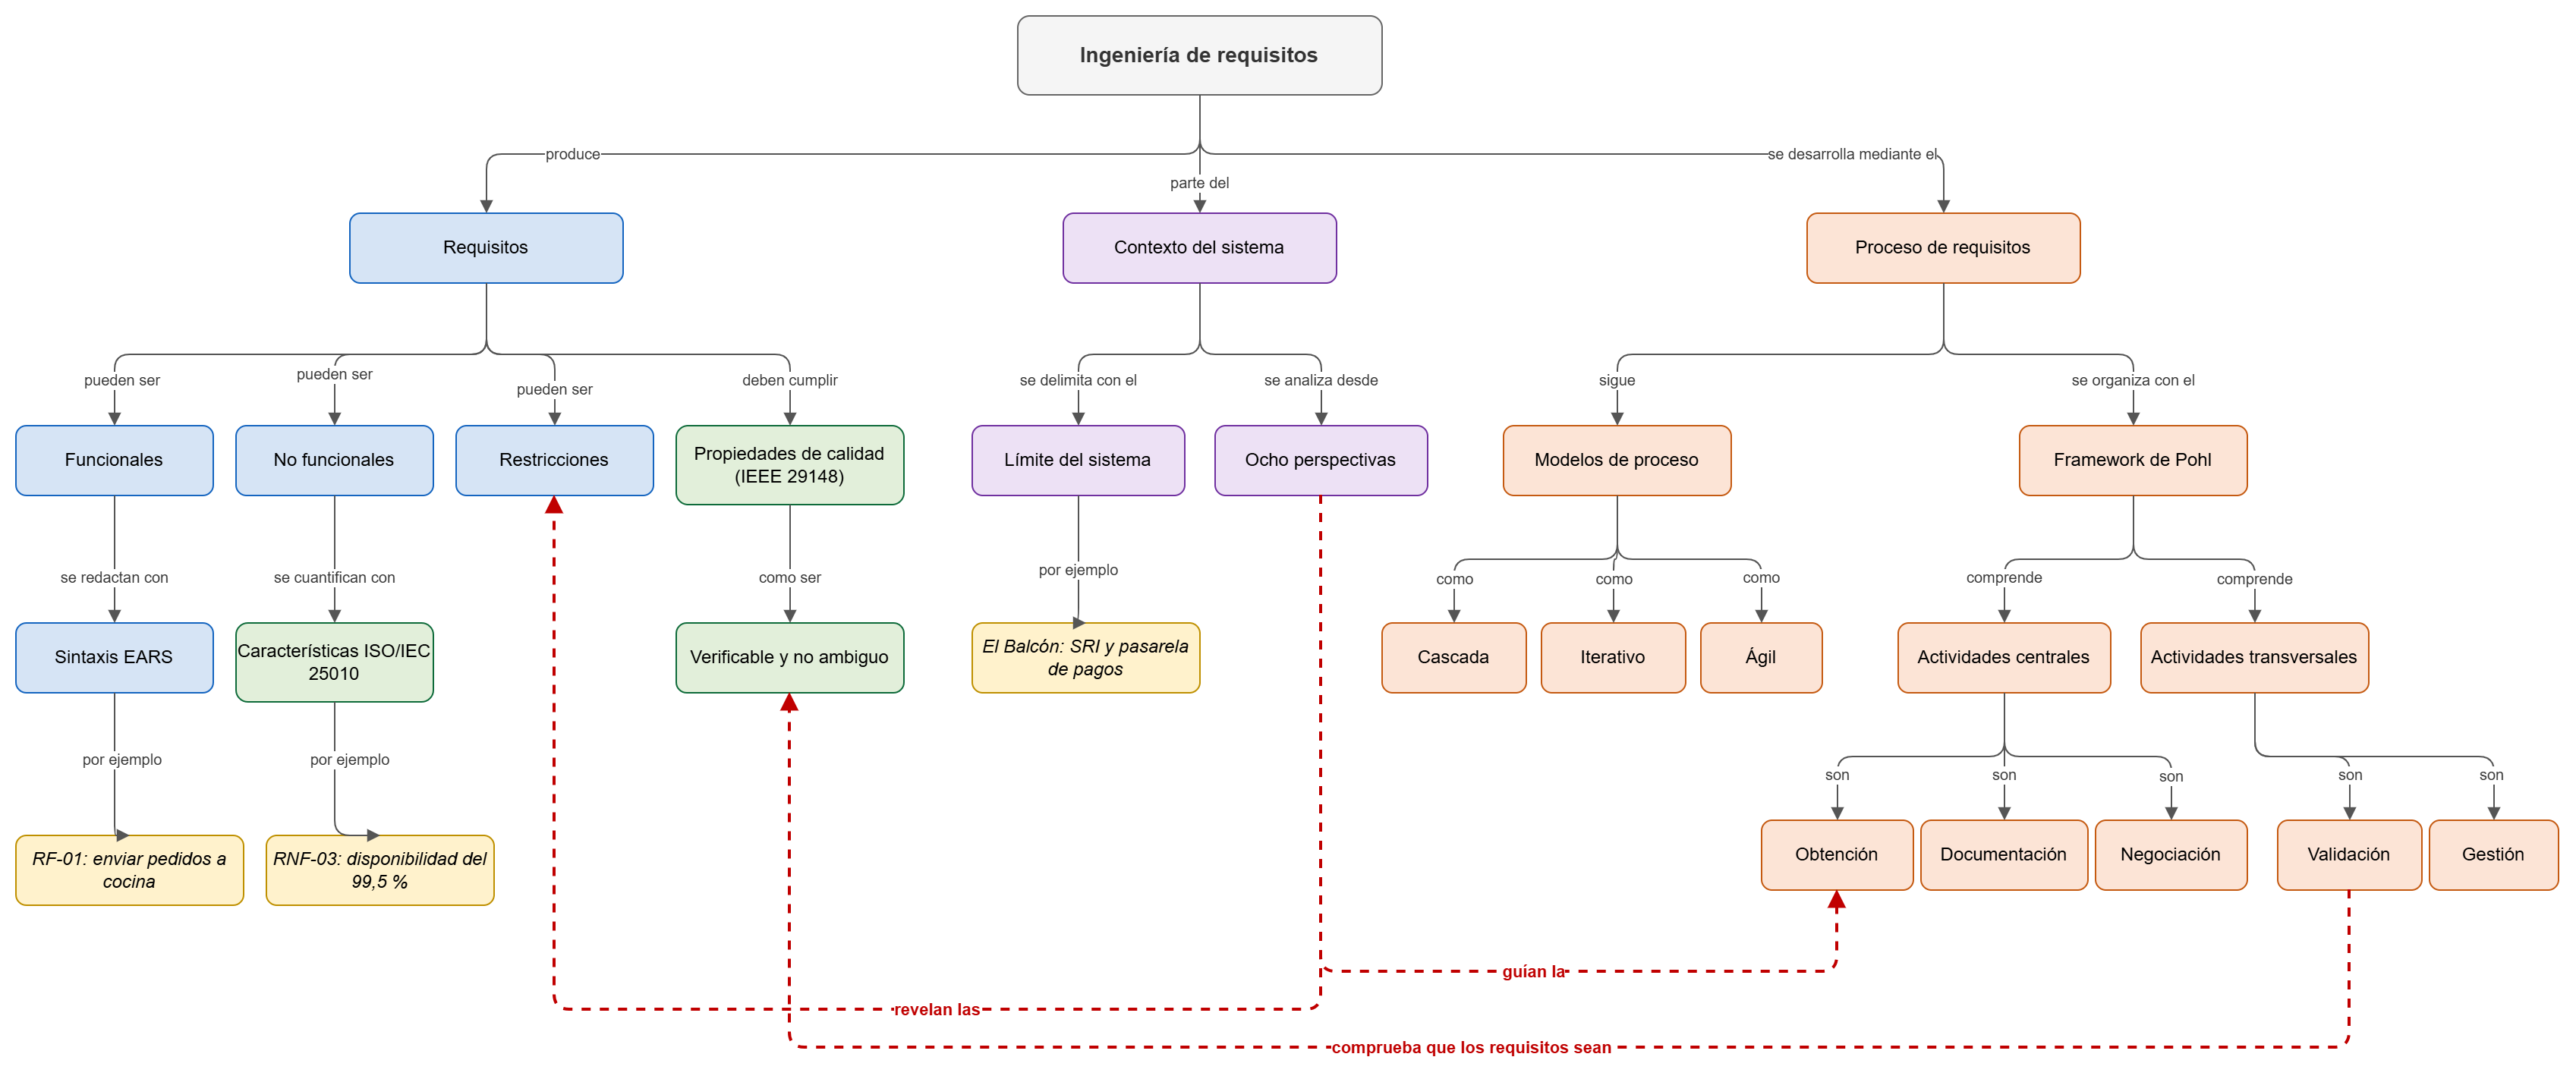
\includegraphics[width=\linewidth,height=0.85\textheight,keepaspectratio]{figuras/mapa-conceptual.png}
\caption{Mapa conceptual integrador de la Unidad 1. Elaborado en draw.io.}
\label{fig:mapa-conceptual}
\end{figure}
\end{landscape}
